\chapter{Marco teórico}
\label{Marco_teorico}

\section{Estudio de mercado}
A lo largo de los años los \ac{RTS} siempre han contado con una gran aceptación entre
los usuarios de \ac{PC}, un claro ejemplo de esto puede ser el juego \textit{`Age of
Empire II: The Age of Kings'}\footnote{Desarrollado por `Ensemble Studios' y lanzado a
finales de 1999.} el cual se posicionó como uno de los juegos más vendidos del momento
superando el millón de copias. Actualmente el juego cuenta con una remasterización
\footnote{Co-desarrollado por Forgotten Empires, Tantalus Media y Wicked
Witch. Lanzado en noviembre de 2019.} la cual ha conseguido vender más de 50.000
copias en \textit{`Steam'}. Datos extraídos de su articulo en \citeauthor*{Wiki_AoE2}.

Si miramos en el panoráma nacional actual, podemos encontar el juego \textit{`They Are
Billions'} \footnote{Desarollado por Numantian Games y lanzado en junio de 2019.}
disponible inicialmente para \ac{PC} y posteriormente lanzado en \textit{`PlayStation 4'}
y \textit{`Xbox One'} debido a su éxito. A día de hoy el juego a conseguido vender
solamente en \textit{`Steam'} más de 25.000 unidades consiguiendo una valoración muy
positiva por parte de los usuarios de la plaforma como podemos ver en la página 
del juego de \citeauthor*{TaB2019} en dicha tienda.

El género puede aparentar ser cosa del pasado pero vistas las cifras podemos concluir
que sigue siendo un reclamo para los jugadores.

\section{Referentes}
A la hora de establecer las mecánicas, el estilo artístico y/o otros aparatados del
juego es habitual basarse o tener en cuenta lo que han hecho otras entregas anteriores
en su momento. Para el desarrollo de este proyecto han sido de gran utilidad una
serie de entregas entre las que cabe destacar dos.

\subsection{Age of Empires II: The Age of Kings}
En primer lugar encontramos el juego \textit{'Age of Empires II: The Age of Kings'}, en
este juego tendremos que gestionar una civilizacion a elegir entre un amplio abanico de
facciones con sus propias unidades y edificaciones.

\begin{figure}[ht]
\centering
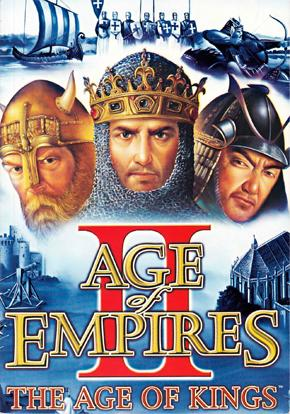
\includegraphics[width=0.3\textwidth]{imagenes/marco_teo/referentes/aoe_1.png}
\caption{Carátula del juego original.}
\label{img:aoe_1}
\end{figure}

El jugador deberá ser capaz de guiar a las unidades, gestionar las ciudades y conseguir
recursos a lo largo del escenario con el fin de derrotar a las demás facciones. Además,
se nos presenta una serie de campañas en las cuales manejaremos a grandes personajes de
la historia como `William Wallace' o `Juana de Arco' entre otros.

El juego hace de referente en varios aspectos entre los que podemos encontrar el
apartado visual donde se utiliza una perspectiva isométrica con cámara fija y el uso
de una estética clásica propia de las épocas a las que pertenecen las civilizaciones.

\begin{figure}[ht]
\centering
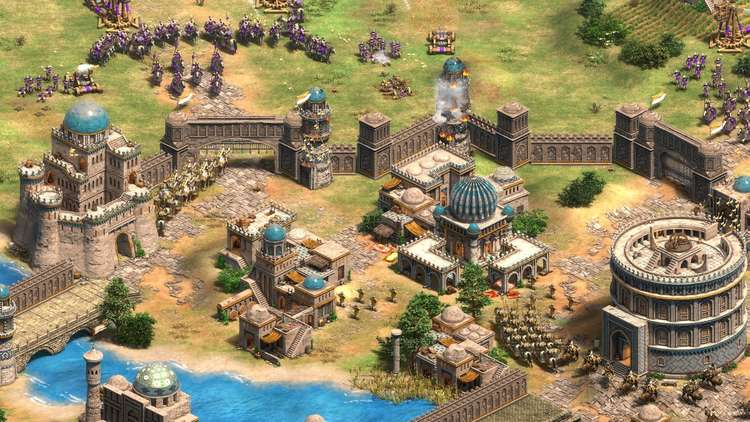
\includegraphics[width=0.7\textwidth]{imagenes/marco_teo/referentes/aoe_2.png}
\caption{Ciudad siendo asediada.}
\label{img:aoe_2}
\end{figure}

Todas la unidades de las que podemos disponer cuentan con una serie características que
las hacen más o menos fuertes en función del objetivo al que ataquen, podemos encontrar
el ejemplo de las máquinas de asedio las cuales son más fuertes contra estructuras pero
más débiles contra infanteria, o las unidades a caballo que son fuertes contra arqueros
e infanteria pero débiles frente a lanceros.
Este tipo de mécanicas dotan al juego de una importante componente táctica en el manejo
de las unidades que debemos dominar si queremos completar los diferentes niveles de
forma satisfactoria~\ref{img:aoe_2}.

\subsection{The Are Billions}
En segundo lugar podemos encontrar el juego \textit{'\acf{TaB}'} el cual reutiliza
una serie de características propias del género y como pueden ser la perspectiva
isométrica pero sin dejar de innovar introduciendo nuevas mecánicas y/o formas de
plantear la jugabilidad.

\begin{figure}[ht]
\centering

\includegraphics[width=0.7\textwidth]{imagenes/marco_teo/referentes/tab_1.png}
\caption{Imágen promocional del juego.}
\label{img:tab_1}
\end{figure}
 
En \textit{'\ac{TaB}'} podemos encontrar funciones interesantes como la pausa
táctica la cual nos permitirá visualizar detenidamente el estado del mapa sin tener que
preocuparnos por no estar atendiendo algunos posibles eventos como ataques a nuestras
tropas por parte del enemigo. En juegos anteriores como los \textit{'\ac{AoE}'} es
fácil encontrarnos en la situación de tener trabajadores en la ciudad sin hacer tareas
un rato y no poder mirar cuales son e ir pensando su ocupación siguiente por estar
atrapado en refriegas con otros jugadores, con este tipo de mecánicas estas situaciones
se solventan en mayor o menor medida y permiten al jugador tomarse el tiempo que
necesite para pensar las acciones que quiere realizar.

Otro aspecto llamativo en el podemos fijarnos es en la aparición de solamente dos
facciones. Por un lado encontramos `El Nuevo Imperio', la facción del jugador, la
cual representa una serie de colonias que tendremos que desarrollar a lo largo de
los niveles. En el otro lado encontramos las infinitas hordas de zombis que tratarán
de exterminar a la raza humana.

\begin{figure}[ht]
\centering
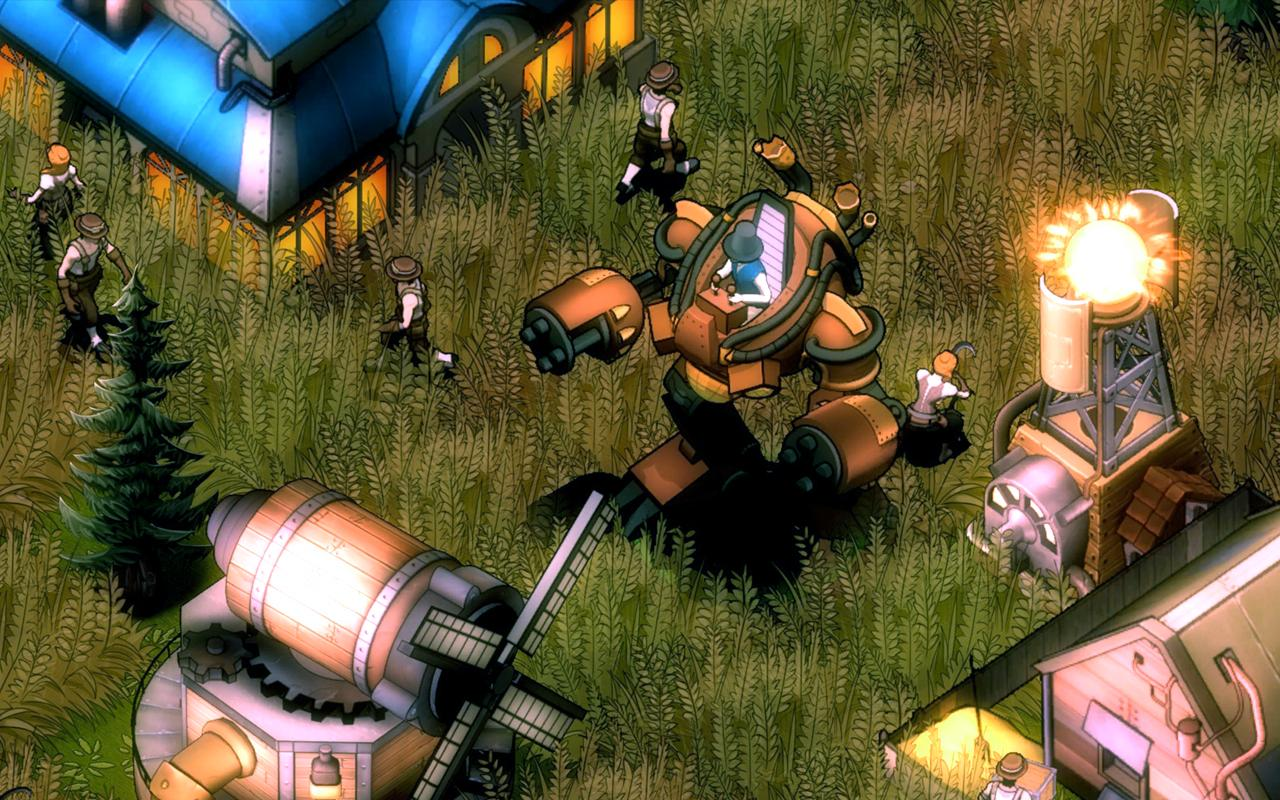
\includegraphics[width=0.6\textwidth]{imagenes/marco_teo/referentes/tab_2.png}
\caption{Ejemplo de unidad mecánica del imperio y estética del juego}
\label{img:tab_2}
\end{figure}

A diferencia de en \textit{'\ac{AoE}'} que todas la facciones poseen las mismas unidades
\footnote{Algunos valores pueden variar según bonos de facción}, en
\textit{'\ac{TaB}'} cada facción dispondrá de unidades únicas con acciones propias.
Como podemos ver en la imágen~\ref{img:tab_2} las tropas del imperio se basan en el uso
de maquinaria y armas de fuego para repeler las hordas enemigas, por otro lado los
zombis contarán con diversas caraterísticas físicas mejoradas conforme sean de mayor
``nivel'' puediendo encontrar algunos más rápidos, o más fuertes o más grandes y
resistentes al daño.~\ref{img:tab_3}

\begin{figure}[ht]
\centering
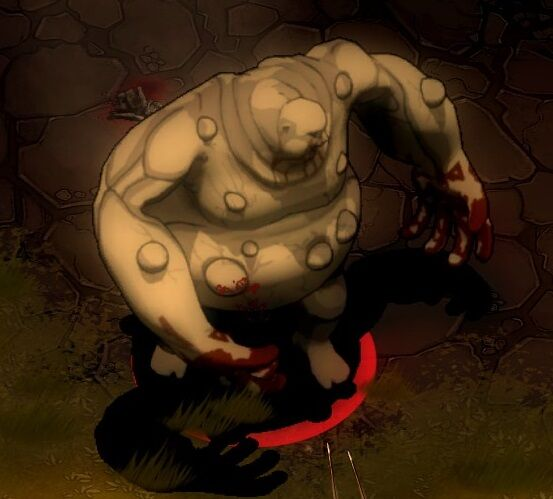
\includegraphics[width=0.5\textwidth]{imagenes/marco_teo/referentes/tab_3.png}
\caption{Infectado gigante}
\label{img:tab_3}
\end{figure}

Como último punto a destacar de la entrega tenemos la introducción del un modo de
juego de supervivencia donde a lo largo del tiempo irán apareciendo oleadas de zombis
donde cada vez aparecen más enemigos y más poderosos de forma infinita, haciendo así
que la partida termine cuando el jugador deje de aguantar la ofensiva enemiga.


\section{Técnicas de inteligencia articificial}
Como ya se ha mencionado anteriormente en la introducción~\ref{intro} de este \ac{TFG}
el grueso del desarrollo y uno de los objetivos más importantes del proyecto recaen en
el desarrollo de una \ac{IA} haciendo uso de las técnicas de \textit{'Flocking'} y
\textit{`Steering behaviors'}.

Para ello nos basaremos principalmente en las explicaciones y ejemplos que podemos
encontrar en el libro \cite[ch.~3]{Millington2009} donde de forma extensa y detallada
se nos introduce en la teoría relacionada a los algoritmos y la forma en la que estos
se estructuran e interactuan entre ellos. Para dar un poco de contexto sobre el tema
resumiremos brevemente las ideas que se nos presentan a lo largo del capitulo dedicado
a estas técnicas. 

Los \textit{`Steering behaviors'} pueden ser entendidos como una serie de algoritmos
destinados a guiar la forma en la cual los \ac{NPC} se desplazan por el escenario
y/o interactuan con los distintos elementos que puedan encontrase en la escena. Siguen
una filosofía de crear movimientos complejos a base de una combinación de movimientos 
y/o acciones simples, un ejemplo común puede ser la acción de perseguir a un objetivo
mientras se sortean obstáculos en el proceso. \\ 
En este caso no tendríamos una función llamada 
\textit{``persigue-enemigo-mientras-esquivas()''} y esta encargarse de todo el 
trabajo, sino que, tendremos el cálculo de la velocidad y dirección necesarias para
alcanzar el objetivo, la compropación para saber si hay algún tipo de
obstáculo por el camino y la rectificación de la trayectoria en caso de
haberlos cada uno por su lado y es la resultante de todos los pasos la que defina el
movimiento final.

Esta forma de estructurar y formar actividades complejas en base a acciones más simples
nos permite reutilizar y jugar con los diferentes comportamientos permitiéndonos crear
con ellos un amplio espectro de resultados.

En lo referente al \textit{'Flocking'} podemos observar como en esencia es lo mismo que
los \textit{`Steering behaviors'} pero añadiendo factores y/o componentes grupales,
el origen del modelo lo podemos encontrar en las publicaciones de \cite{Boids1986} donde
se nos introduce el concepto de \textit{``Boid''} como entidad generica que simula su
comportamiento bajo este algoritmo. Además, se nos introducen los tres comportamientos
básicos en los que se basa la técnica para generar el movimiento emergente, que son:

La \textbf{separación}~\ref{img:separation-b} que cada \textit{Boid} mantendrá entre
las demás entidades en su vencidad, con esto evitaremos solapamientos y respetar el
espacio y movimiento de las demás entidades.

\begin{figure}[ht]
\centering
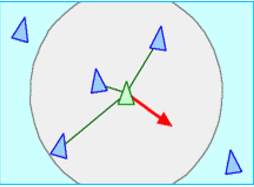
\includegraphics[width=0.35\textwidth]{imagenes/marco_teo/separation.png}
\caption{Separation behavior}
\label{img:separation-b}
\end{figure}

Por otro lado podemos encontrar el \textbf{alineamiento}~\ref{img:alignment-b} de la
dirección del movimento propio con las de las entidades más cercanas, de esta forma conseguimos un
movimiento armónico entre los \textit{boids} y produciremos una sensación de
coordinación entre ellos.

\begin{figure}[ht]
\centering
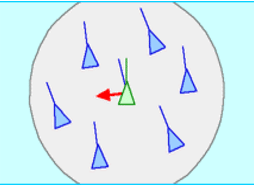
\includegraphics[width=0.35\textwidth]{imagenes/marco_teo/alignment.png}
\caption{Alignment behavior}
\label{img:alignment-b}
\end{figure}

Por último encontramos la \textbf{cohesión}~\ref{img:cohesion-b} la cual se encargará de
mantener a las entidades cercanas juntas para crear esa sensación de grupo que buscamos
con el algoritmo.

\begin{figure}[ht]
\centering
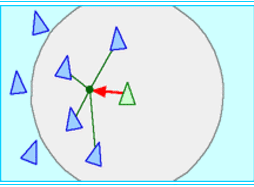
\includegraphics[width=0.35\textwidth]{imagenes/marco_teo/cohesion.png}
\caption{Cohesion behavior}
\label{img:cohesion-b}
\end{figure}

Por otro lado, podemos ver en el articulo de `Raynolds' como a lo largo de los años se
ha ido modificando y ampliando el algoritmo con el fin de añadir variaciones en el
comportamiento y/o introducir más factores influyentes en la decisión de los 
\textit{Boids} como puede ser el olor de determinada entidad/es y/o escenario. \\
Esto sin duda es gracias a la versatílidad que nos proporciona el uso de los
\textit{`Steering behaviors'} y jugar con la importancia de las distintas componentes
a la hora de hacer la toma de decisiones.

